\documentclass[tikz,border=10pt]{standalone}
\begin{document}
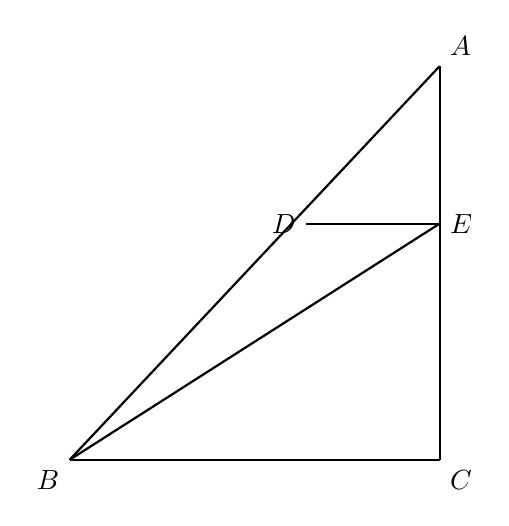
\begin{tikzpicture}[line width=0.8pt, scale=1]
\coordinate (A) at (4.7,5);
\coordinate (B) at (0,0);
\coordinate (C) at (4.7,0);
\coordinate (D) at (3,3);
\coordinate (E) at (4.7,3);

\draw (B) -- (A);
\draw (A) -- (C);
\draw (B) -- (C);
\draw (D) -- (E);
\draw (B) -- (E);

\node[above right] at (A) {$A$};
\node[below left] at (B) {$B$};
\node[below right] at (C) {$C$};
\node[left] at (D) {$D$};
\node[right] at (E) {$E$};
\end{tikzpicture}
\end{document}
